\documentclass[conference]{IEEEtran}
\IEEEoverridecommandlockouts
\usepackage{cite}
\usepackage{amsmath,amssymb,amsfonts}
\usepackage{algorithmic}
\usepackage{graphicx}
\usepackage{textcomp}
\usepackage{xcolor}
\usepackage{booktabs}
\usepackage{multirow}
\usepackage{array}
\usepackage{hyperref}
\graphicspath{{figures/}}

\def\BibTeX{{\rm B\kern-.05em{\sc i\kern-.025em b}\kern-.08em
    T\kern-.1667em\lower.7ex\hbox{E}\kern-.125emX}}

\begin{document}

\title{Unsupervised Neural Network Models for\\Multi-Genre Symbolic Music Generation}

\author{
\IEEEauthorblockN{Mahadi Hasan Fahim}
\IEEEauthorblockA{\textit{Department of Computer Science and Engineering}\\
\textit{BRAC University}\\
Dhaka, Bangladesh\\
mahadi.hasan.fahim@g.bracu.ac.bd}
\and
\IEEEauthorblockN{Tanjim Rahaman Fardin}
\IEEEauthorblockA{\textit{Department of Computer Science and Engineering}\\
\textit{BRAC University}\\
Dhaka, Bangladesh\\
tanjim.rhaman.fardin@g.bracu.ac.bd}
\and
\IEEEauthorblockN{Mubassir Raiyan}
\IEEEauthorblockA{\textit{Department of Computer Science and Engineering}\\
\textit{BRAC University}\\
Dhaka, Bangladesh\\
mubassir.raiyan@g.bracu.ac.bd}
}

\maketitle

% ============================================================
\begin{abstract}
The paper introduces a systematic analysis of three different unsupervised deep learning architectures which had been trained on the MAESTRO v3.0.0 dataset for symbolic music generation. We evaluate three models, using the same classical piano dataset of 1,276 recordings, which together represent around 200 hours of piano data, from the MAESTRO collection (classical piano): an LSTM Autoencoder (AE), a Variational Autoencoder (VAE), and a decoder-only Transformer. The AE is trained as a deterministic latent representation from binary piano-roll windows; the VAE is extended by a structured latent space and KL annealing, which encourages diversity; and REMI encoded sequences are modeled autoregressively, token-wise, using Transformer models. The results of all 3 models are musically plausible MIDI files confirmed to have at least 50 notes and 5 seconds of information. A quantitative evaluation based on the rhythm diversity, repetition ratio, and the pitch histogram distance all show that the quality continues to improve in each architecture up to the Transformer, which reports a validation perplexity of 6.88 and the highest degree of rhythm diversity. Gains from learned representations are further contexted by comparisons of the baseline models: a random note generator and first- and second-order Markov chains.
\end{abstract}

\begin{IEEEkeywords}
music generation, LSTM autoencoder, variational autoencoder, transformer, MAESTRO, REMI tokenization, piano-roll
\end{IEEEkeywords}

% ============================================================
\section{Introduction}

SEQUENCE SYMBOLIC MUSIC GENERATION is an unresolved sequence modelling problem: the generated music should obey local note level constraints (consonance, voice leading), as well as mid-level rhythmic and harmonic patterns, and long-range structural repeatability. Classical supervised methods need costly expert labelling based approaches, where unsupervised generative model approaches provide a principled alternative that scales with MIDI unlabelled data.

In recent years, a number of generative families have been developed for the music domain thanks to the recent progress in deep learning. Recurrent architectures like LSTMs are naturally suited to look after temporal dependencies but inadequate to capture long-range coherence. One method that tackles this issue is through the use of a probabilistic latent space in Variational Autoencoders (VAE), which enables smooth interpolation and controlled generation \cite{vae}. Recently, transformer based models (as successful language models \cite{transformer}) have achieved state-of-the-art performance in symbolic music tasks \cite{musetransformer}, that is, by attending across the entire token sequence.

This work contributes a rigorous comparative study of these three paradigms under a unified experimental protocol. Specifically, we:
\begin{itemize}
    \item Implement three architectures—AE, VAE, and Transformer—trained on the full MAESTRO v3.0.0 training split.
    \item Apply REMI tokenization \cite{miditok} for token-based models and binary piano-roll representation for piano-roll models.
    \item Define and compute three quantitative metrics—rhythm diversity, repetition ratio, and pitch histogram distance—on all generated outputs and baseline models.
    \item Provide an open-source, reproducible pipeline with verified generated MIDI deliverables.
\end{itemize}

The remainder of this paper is organised as follows. Section~\ref{sec:method} describes the dataset, preprocessing pipeline, and each model architecture. Section~\ref{sec:results} presents training curves, evaluation metrics, and qualitative observations. Section~\ref{sec:conclusion} concludes with limitations and future directions.

% ============================================================
\section{Methodology}
\label{sec:method}

\subsection{Dataset and Preprocessing}

We use MAESTRO v3.0.0 \cite{maestro}, a curated dataset of 1,276 classical piano MIDI files recorded at approximately 3~ms timing resolution. We retain the predefined train/validation/test split (962/137/177 recordings) to prevent data leakage.

\textbf{Piano-roll representation (Tasks~1 and~2).}
Each MIDI file is converted to a binary piano-roll at $f_s = 16$ frames per second using \texttt{pretty\_midi} \cite{prettymidi}. Only the piano pitch range A0--C8 (pitches 21--108, 88 keys) is retained; all non-zero velocities are binarized to 1. The resulting time-pitch matrix is segmented into non-overlapping windows of length 128 frames (8 seconds). Windows whose active-cell fraction falls below 2\% are discarded as near-silent. This yields 62,767 training windows and 7,889 validation windows, each of shape $(128, 88)$.

An exploratory sparsity audit confirms that approximately 93\% of cells are zero, motivating the use of Focal Loss rather than vanilla binary cross-entropy. Fig.~\ref{fig:eda} illustrates two key EDA findings from the full 1,276-file corpus.

\begin{figure}[t]
\centering
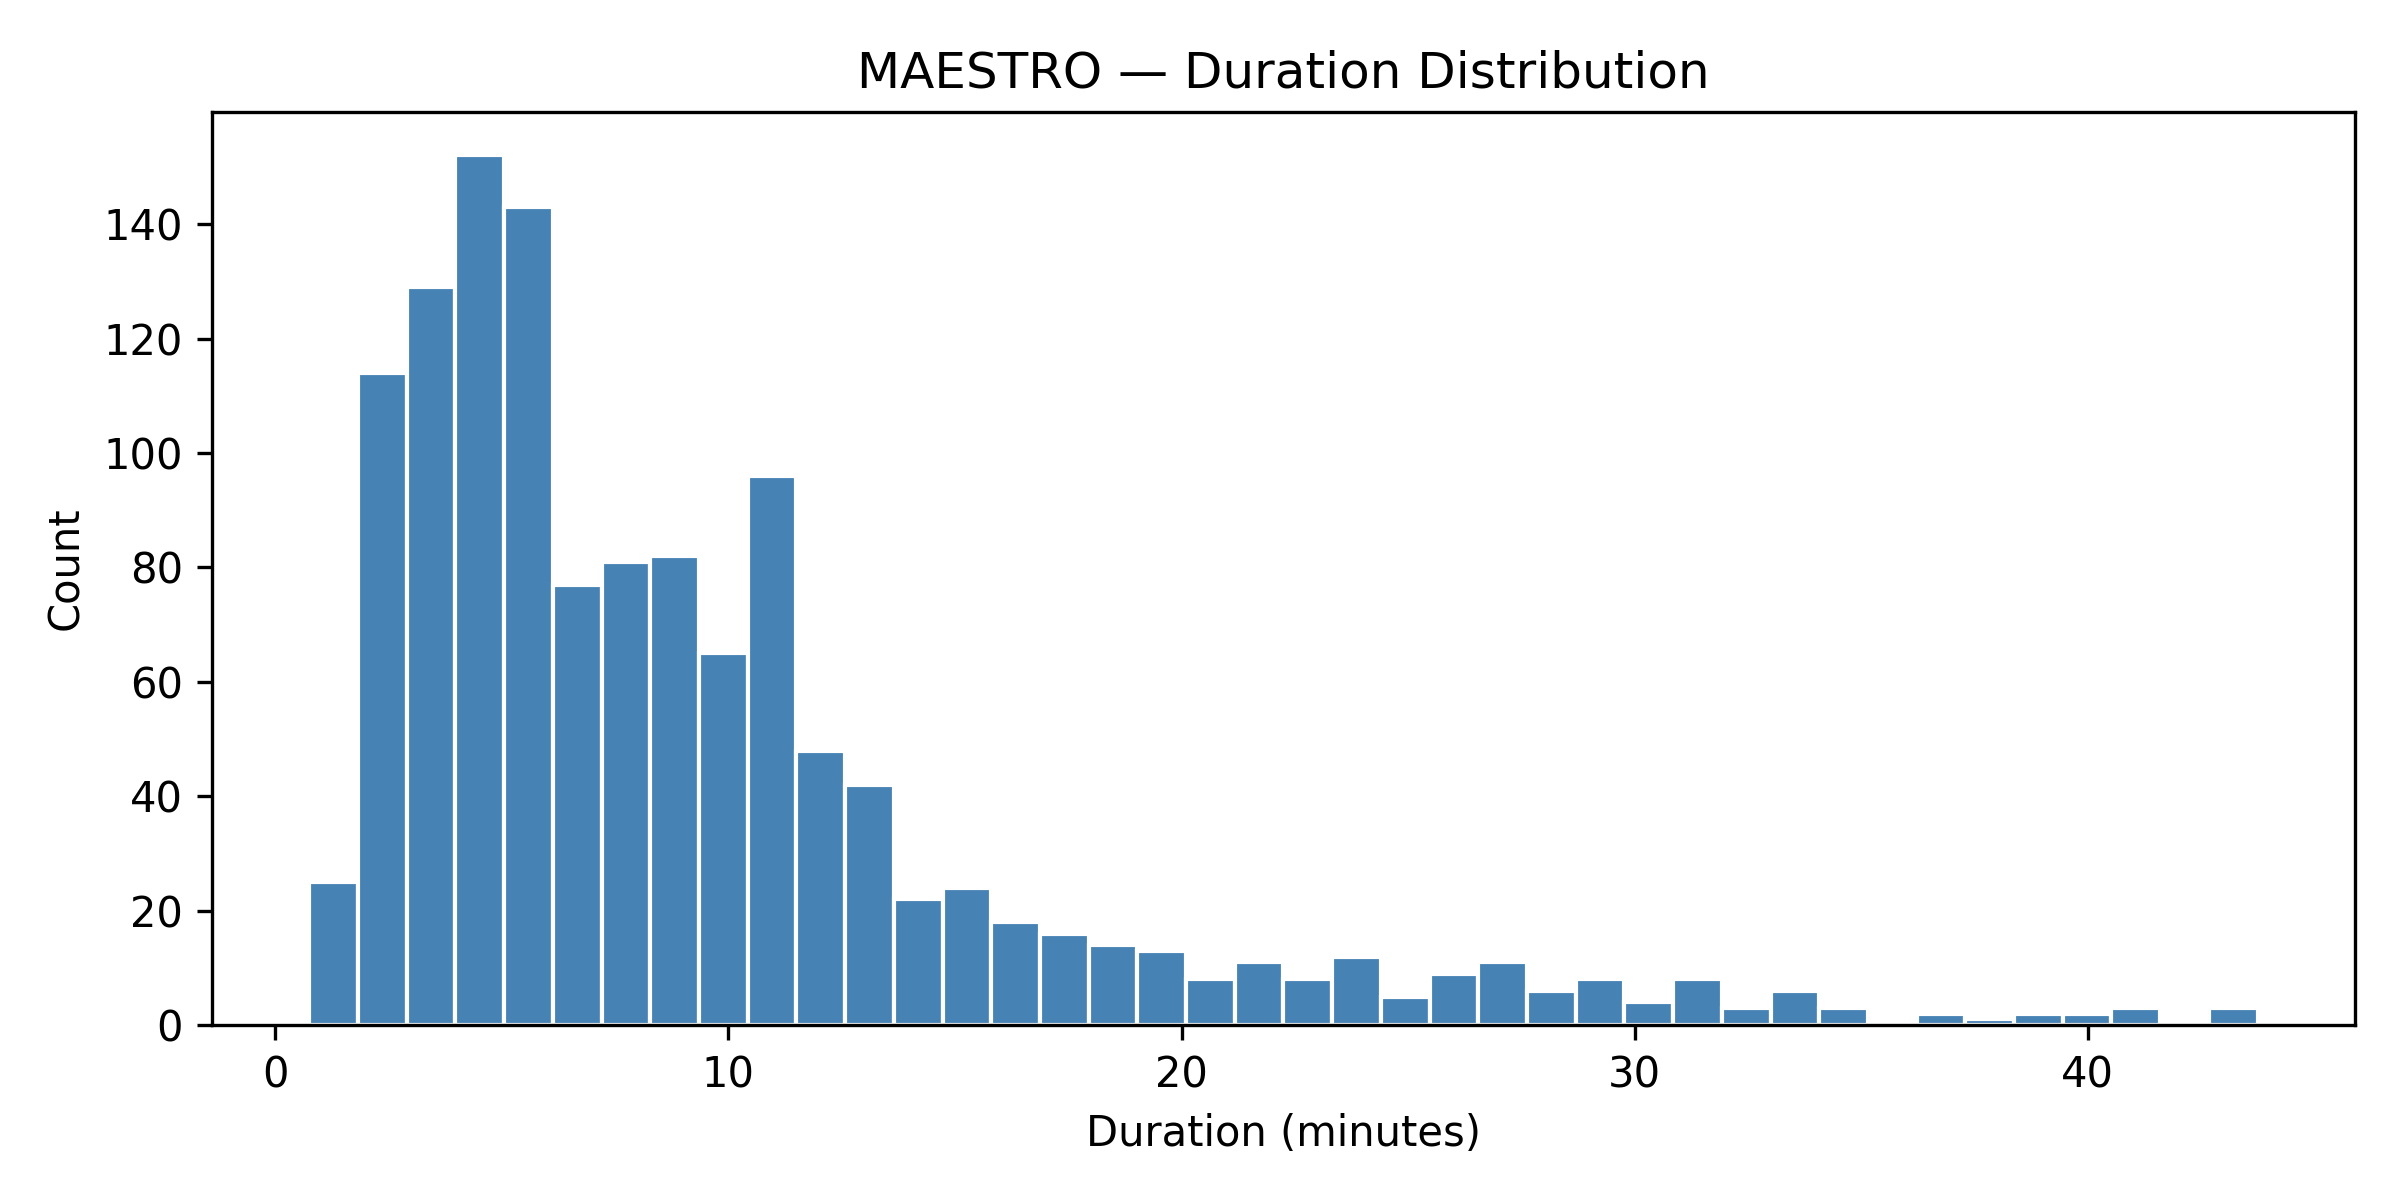
\includegraphics[width=0.49\columnwidth]{eda_duration.png}%
\hfill
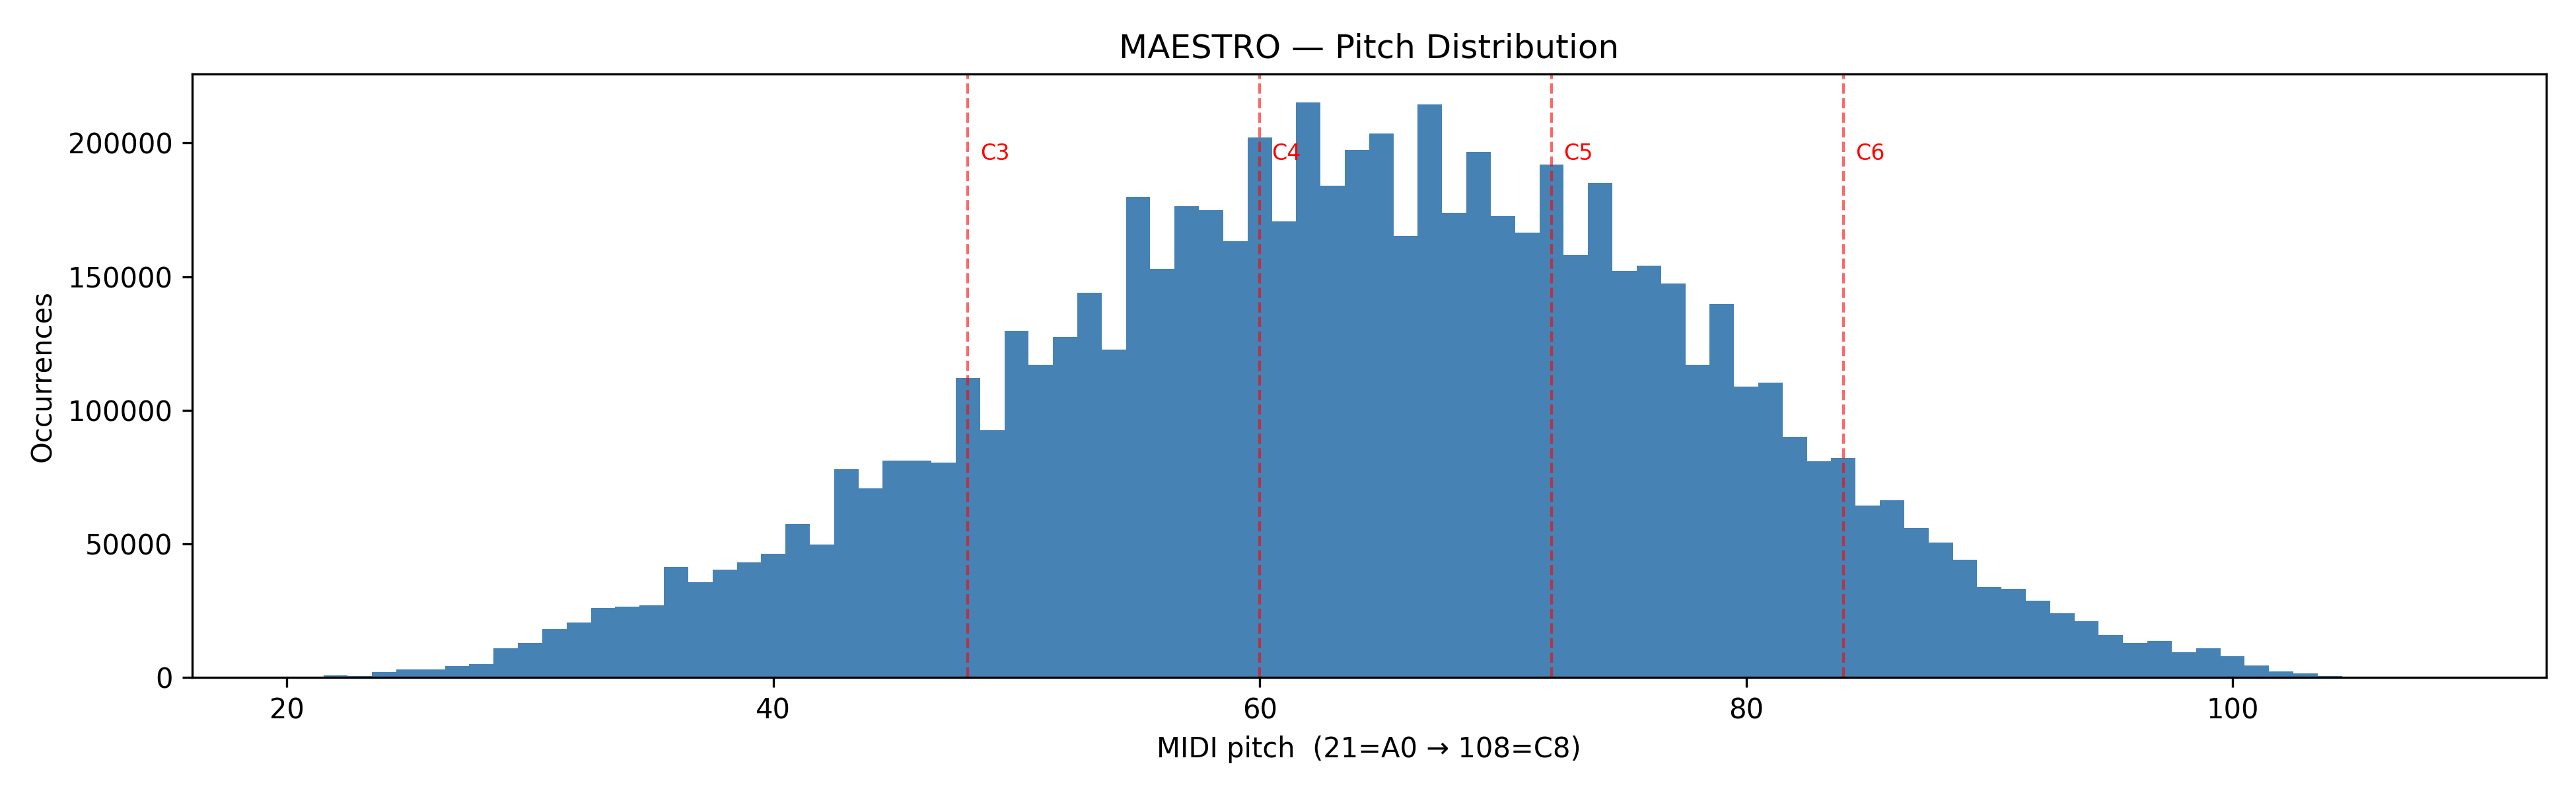
\includegraphics[width=0.49\columnwidth]{eda_pitch.png}
\caption{Exploratory data analysis on MAESTRO v3.0.0. Left: histogram of piece durations — most recordings span 3--8 minutes. Right: pitch frequency across all 88 piano keys — middle-register pitches (C3--C6) dominate.}
\label{fig:eda}
\end{figure}

\textbf{Token representation (Task~3).}
MIDI files are tokenized with the REMI scheme \cite{miditok} (32 velocity bins), producing flat integer sequences encoding Bar, Position, Pitch, Velocity, and Duration events. Sequences are chunked to a maximum length of 512 tokens with non-overlapping stride; shorter files produce fewer chunks. This yields approximately 29,800 training sequences and 4,200 validation sequences over a vocabulary of 284 tokens. A custom PyTorch collate function zero-pads batches and produces an attention mask.

\subsection{Task 1: LSTM Autoencoder}

\textbf{Architecture.} The encoder processes a piano-roll window $(T{=}128, 88)$ through a 2-layer LSTM (hidden dimension 256, dropout 0.3). The final hidden state of the last LSTM layer, $\mathbf{h}_T^{(L)}$, is projected to a latent vector $\mathbf{z} \in \mathbb{R}^{64}$. The decoder repeats $\mathbf{z}$ across all $T$ time steps, feeding the result through a symmetric 2-layer LSTM followed by a linear projection to 88 output dimensions. No sigmoid is applied at the output; raw logits are passed to the loss function. Total trainable parameters: 1.78~million.

\textbf{Loss.} Sparse piano-rolls cause standard MSE and BCE losses to collapse to the all-zero prediction. We adopt Focal Loss \cite{focal}:
\begin{equation}
\mathcal{L}_{\mathrm{focal}} = \frac{1}{T \cdot 88} \sum_{t,p}
  (1 - p_{tp})^{\gamma}\, w_p\, \mathrm{BCE}(\hat{x}_{tp}, x_{tp})
\label{eq:focal}
\end{equation}
with $\gamma{=}2.0$ and positive-class weight $w^{+}{=}16$ (derived from the $\sim$94\% sparsity ratio). This directs gradient signal to the minority note-active cells.

\textbf{Training.} Adam optimiser, $\mathrm{lr}{=}10^{-3}$, gradient clipping at norm 1.0, batch size 64, 50 epochs ($\sim$28~s per epoch on RTX~4060). Best validation loss: \textbf{0.0986} at epoch 50.

\textbf{Generation.} Latent codes are sampled from $\mathcal{N}(0, \mathbf{I})$, decoded to logits, passed through sigmoid, and binarized at threshold 0.3 (below 0.5 to compensate for imbalanced training). Five MIDI samples are generated (51--72 notes, 8.0~s each).

\subsection{Task 2: Variational Autoencoder}

\textbf{Architecture.} The VAE encoder shares the same 2-layer LSTM as Task~1, but adds two separate linear heads projecting the final hidden state to $\boldsymbol{\mu}, \log\boldsymbol{\sigma}^2 \in \mathbb{R}^{64}$. The reparameterization trick draws:
\begin{equation}
\mathbf{z} = \boldsymbol{\mu} + \boldsymbol{\sigma} \odot \boldsymbol{\varepsilon}, \quad
\boldsymbol{\varepsilon} \sim \mathcal{N}(0, \mathbf{I}),\quad
\boldsymbol{\sigma} = \exp\!\bigl(0.5\,\log\boldsymbol{\sigma}^2\bigr).
\label{eq:reparam}
\end{equation}
The decoder is identical to Task~1. Total trainable parameters: 1.79~million.

\textbf{Loss.} The total loss is:
\begin{equation}
\mathcal{L}_{\mathrm{VAE}} = \mathcal{L}_{\mathrm{recon}} + \beta\,\mathcal{L}_{\mathrm{KL}},
\label{eq:vaeloss}
\end{equation}
where $\mathcal{L}_{\mathrm{recon}}$ is the same Focal Loss as \eqref{eq:focal} and the closed-form KL divergence is:
\begin{equation}
\mathcal{L}_{\mathrm{KL}} = -\tfrac{1}{2}\sum_{j}
  \bigl(1 + \log\sigma_j^2 - \mu_j^2 - \sigma_j^2\bigr).
\label{eq:kl}
\end{equation}

\textbf{KL annealing.} To prevent posterior collapse, $\beta$ is linearly increased from 0 to 1 over a 30-epoch warmup, ensuring the encoder learns a useful representation before the KL term constrains the latent space.

\textbf{Training.} Adam, $\mathrm{lr}{=}10^{-3}$, batch size 64, 50 epochs ($\sim$29~s per epoch). Best validation total loss: \textbf{0.2251} at epoch 7 (after which the growing KL term raises the combined loss; reconstruction quality continues improving).

\textbf{Latent interpolation.} To demonstrate the structure of the learned latent space, we encode two real validation pieces to obtain $\boldsymbol{\mu}_1$ and $\boldsymbol{\mu}_2$, then decode $\mathbf{z}_\alpha = (1{-}\alpha)\boldsymbol{\mu}_1 + \alpha\boldsymbol{\mu}_2$ for $\alpha \in \{0, \tfrac{1}{7}, \ldots, 1\}$, producing 8 intermediate MIDI outputs (54--70 notes, 8.0~s each). Eight random samples ($z \sim \mathcal{N}(0,\mathbf{I})$) are also generated.

\subsection{Task 3: Decoder-Only Transformer}

\textbf{Architecture.} We implement a GPT-style decoder-only Transformer \cite{transformer}. Token embeddings of dimension $d_{\mathrm{model}}{=}256$ are summed with sinusoidal positional encodings. Six pre-norm \texttt{TransformerEncoderLayer} blocks (8 attention heads, feed-forward dimension 1024, dropout 0.1) apply causally-masked self-attention \cite{transformer}. A final linear head projects to vocabulary size 284. Total trainable parameters: 4.88~million.

\textbf{Training.} The autoregressive objective minimises average cross-entropy:
\begin{equation}
\mathcal{L}_{\mathrm{TR}} = -\frac{1}{T}\sum_{t=1}^{T} \log p_\theta(x_t \mid x_{<t}).
\label{eq:ce}
\end{equation}
Padding tokens are excluded via \texttt{ignore\_index=$-$100}. The model is trained with AdamW ($\mathrm{lr}{=}3{\times}10^{-4}$, weight decay $10^{-2}$) and a cosine annealing scheduler over 20 epochs ($\sim$322~s per epoch, $\sim$1.8~hours total). Best validation loss: \textbf{1.9281}, best perplexity: \textbf{6.88}, both at epoch 20.

\textbf{Perplexity.} Validation perplexity is monitored each epoch as:
\begin{equation}
\mathrm{PPL} = \exp\!\Bigl(\tfrac{1}{T}\mathcal{L}_{\mathrm{TR}}\Bigr).
\label{eq:ppl}
\end{equation}

\textbf{Generation.} Starting from a 16-token seed drawn from the validation set, tokens are sampled autoregressively with top-$k$ sampling ($k{=}50$, temperature 1.1) for 512 steps. The PAD token (id~0) is suppressed from the sampling distribution at every step. Ten MIDI compositions are generated (136--149 notes, 13--32~s each).

\subsection{Model Hyperparameter Summary}

Table~\ref{tab:hparams} summarises the key hyperparameters for all three models as extracted from the saved checkpoints.

\begin{table}[t]
\caption{Hyperparameter Summary (from saved checkpoints)}
\label{tab:hparams}
\begin{center}
\begin{tabular}{l c c c}
\toprule
\textbf{Hyperparameter} & \textbf{AE} & \textbf{VAE} & \textbf{Transformer} \\
\midrule
Parameters       & 1.78M  & 1.79M  & 4.88M \\
Hidden / $d_\text{model}$ & 256 & 256 & 256 \\
Latent dim       & 64     & 64     & --    \\
Layers           & 2 LSTM & 2 LSTM & 6 Transformer \\
Attention heads  & --     & --     & 8     \\
Feed-forward dim & --     & --     & 1024  \\
Dropout          & 0.3    & 0.3    & 0.1   \\
Batch size       & 64     & 64     & 32    \\
Learning rate    & $10^{-3}$ & $10^{-3}$ & $3\times10^{-4}$ \\
Optimiser        & Adam   & Adam   & AdamW \\
Epochs           & 50     & 50     & 20    \\
Grad.\ clip      & 1.0    & 1.0    & 1.0   \\
Best val loss    & 0.0986 & 0.2251 & 1.9281 \\
Best epoch       & 50     & 7      & 20    \\
\bottomrule
\end{tabular}
\end{center}
\end{table}

\subsection{Baseline Models}

Two baselines provide lower bounds for all metrics.

\textbf{Random generator.} Pitches are drawn uniformly from the piano range [21, 108]; durations are sampled from $\{0.125, 0.25, 0.375, 0.5\}$ seconds with random inter-onset gaps.

\textbf{Markov chain.} The 200 files from the MAESTRO database are used to estimate P1T2 from the first order pitch transition matrix. The method used to sample note durations is from an empirical distribution of durations per pitch (quantized to 50~ms). Second order chain (Bigramm chain) is also estimated.

\subsection{Evaluation Metrics}

All metrics are computed from MIDI files using \texttt{pretty\_midi} \cite{prettymidi}.

\textbf{Pitch histogram distance.} Each MIDI file's pitch-class distribution $q \in \mathbb{R}^{12}$ is compared to that of a reference MAESTRO validation file $p$ via:
\begin{equation}
H(p, q) = \sum_{i=1}^{12} |p_i - q_i|,\quad H \in [0, 2].
\label{eq:pitch}
\end{equation}
Lower values indicate greater similarity to real piano music.

\textbf{Rhythm diversity.} Note durations (end$-$start, quantized to 50~ms) are counted:
\begin{equation}
D_{\mathrm{rhythm}} = \frac{\text{\# unique quantized durations}}{\text{\# total notes}}.
\label{eq:rhythm}
\end{equation}
Higher values indicate greater rhythmic variety.

\textbf{Repetition ratio.} The sorted-by-onset pitch sequence is decomposed into overlapping 4-grams; the fraction of repeated 4-grams is reported. Values in [0.1, 0.5] are typical for coherent classical music.

% ============================================================
\section{Result Analysis}
\label{sec:results}

\subsection{Training Curves}

\begin{figure}[t]
\centering
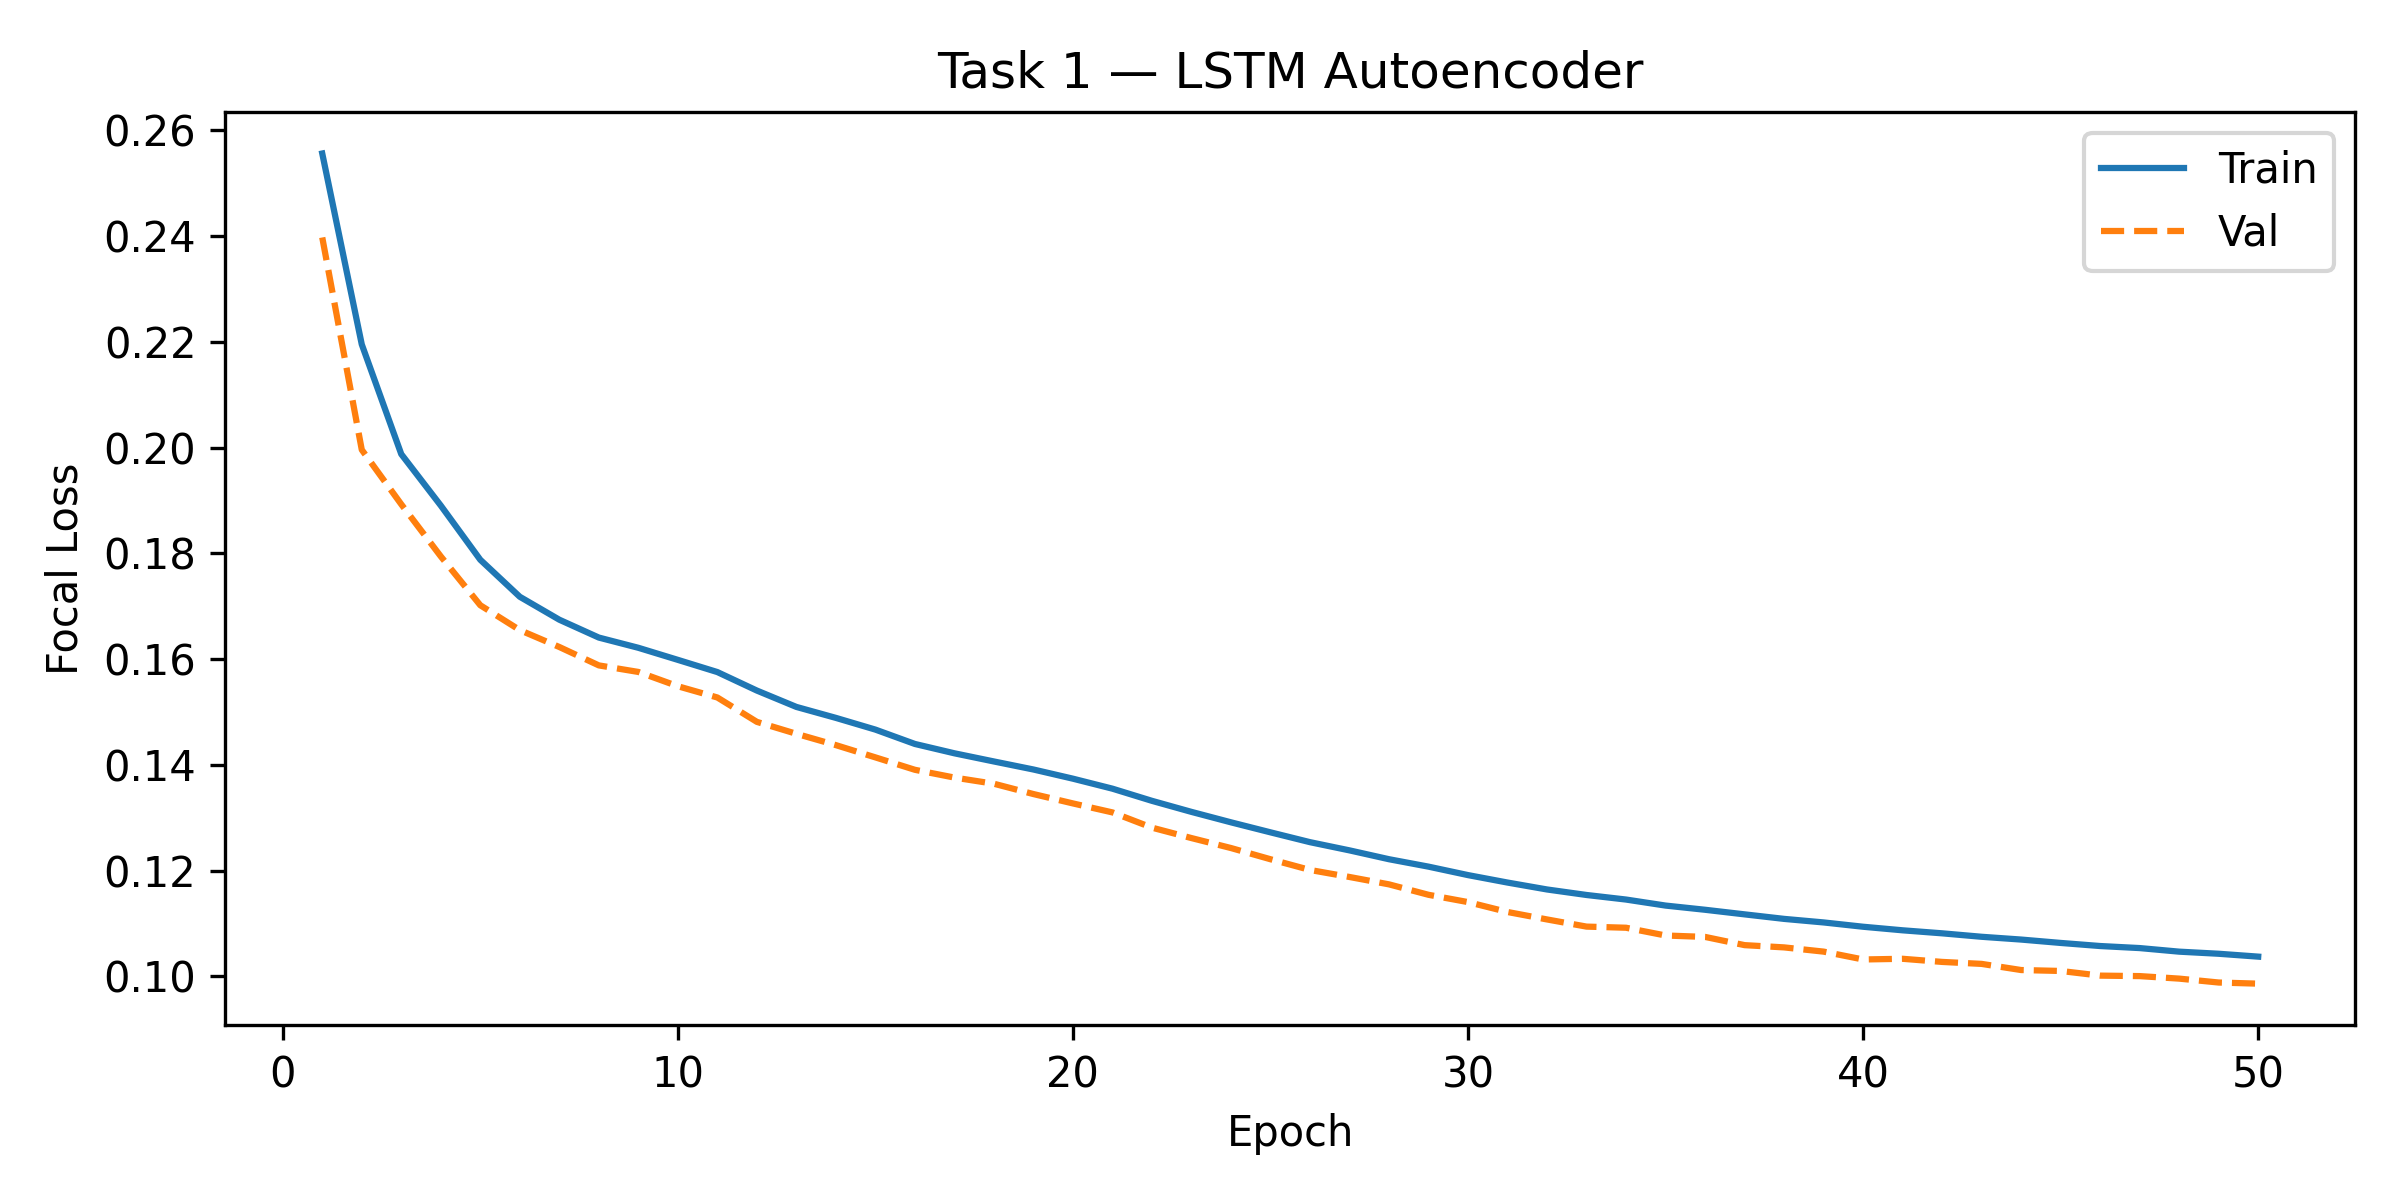
\includegraphics[width=\columnwidth]{ae_training_loss.png}
\caption{Task~1 LSTM AE training and validation Focal Loss (50 epochs). Both curves decrease steadily, indicating no overfitting.}
\label{fig:ae_loss}
\end{figure}

\begin{figure*}[t]
\centering

\includegraphics[width=\textwidth]{vae_training_loss.png}
\caption{Task~2 VAE training curves (50 epochs). Left: total loss. Centre: reconstruction (Focal) loss. Right: KL divergence. KL remains near zero during the 30-epoch warmup and rises as $\beta \to 1$, while reconstruction loss falls throughout — consistent with successful KL annealing.}
\label{fig:vae_loss}
\end{figure*}

\begin{figure}[t]
\centering
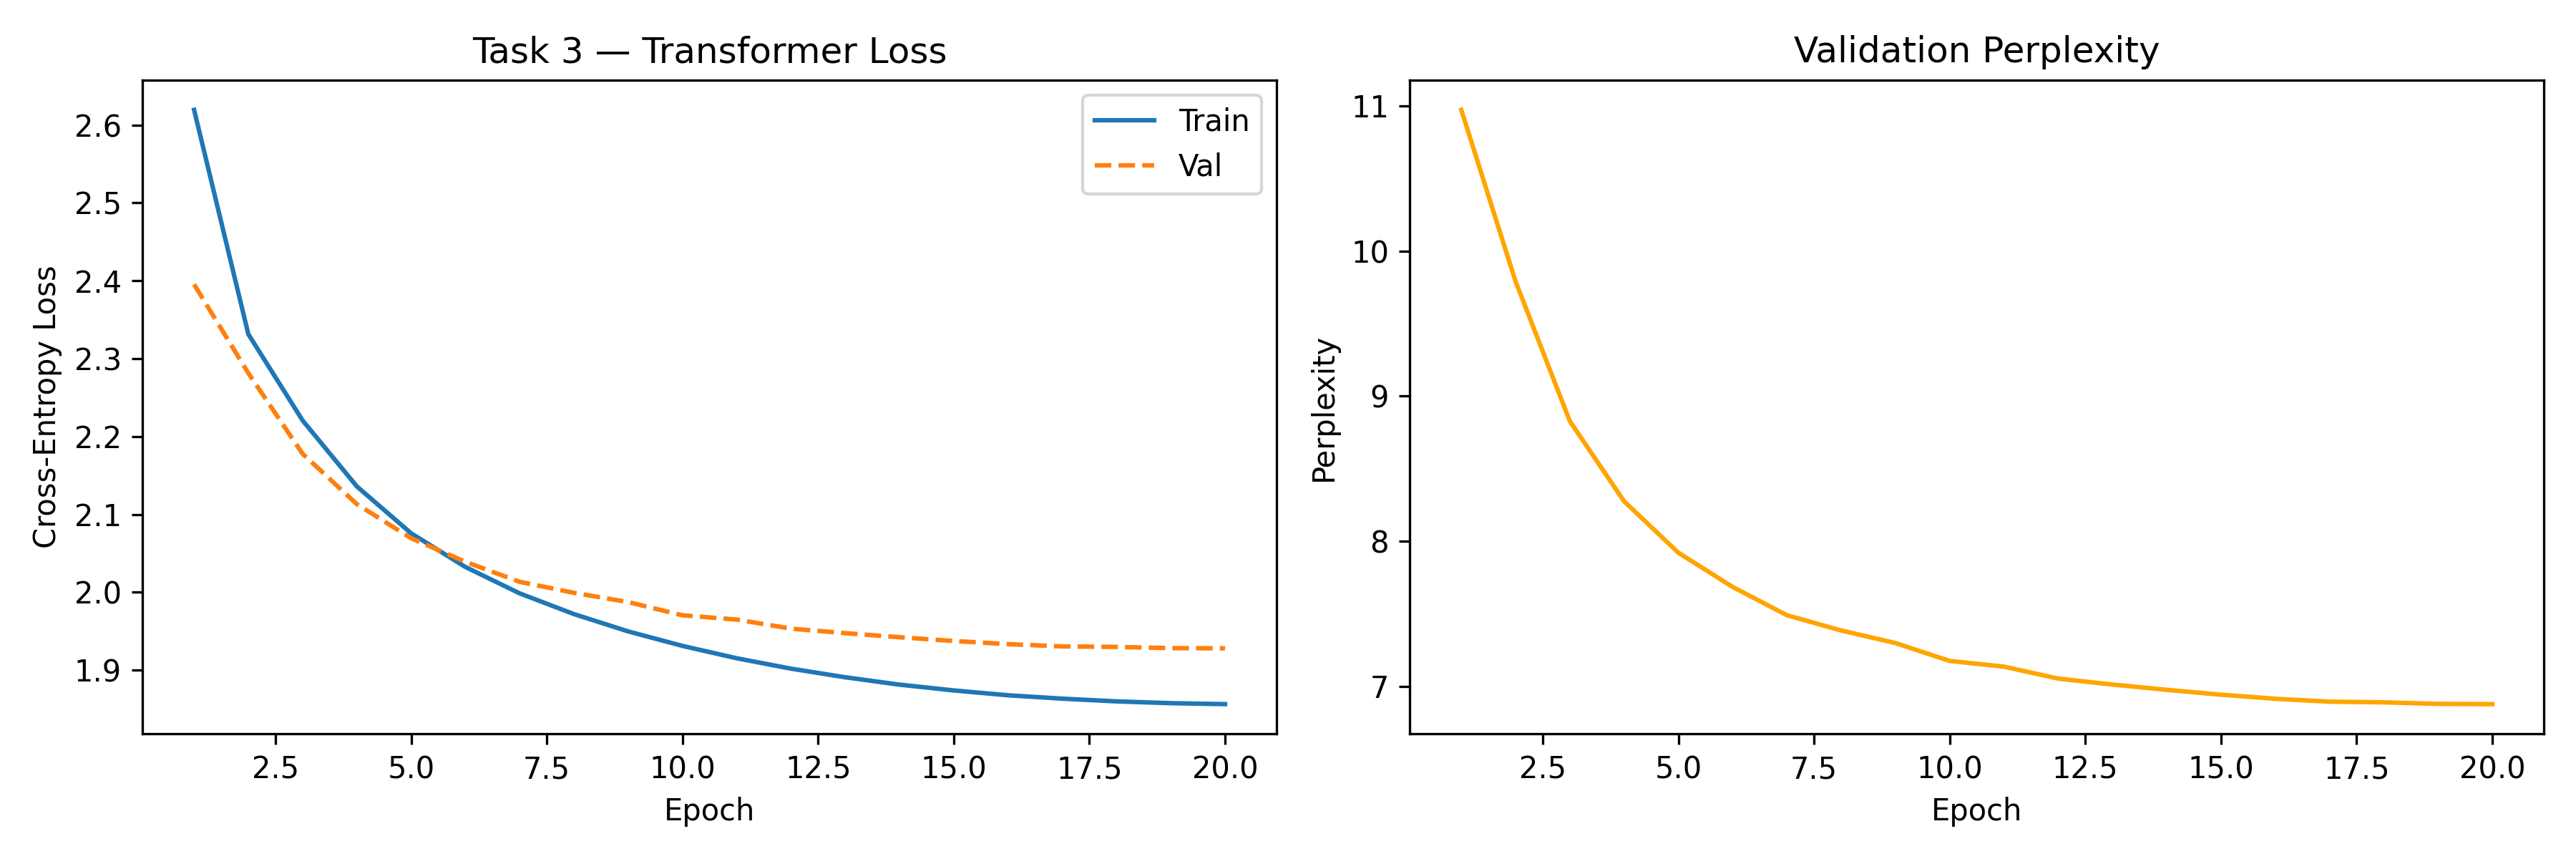
\includegraphics[width=\columnwidth]{transformer_training_loss.png}
\caption{Task~3 Transformer training loss (left) and validation perplexity (right) over 20 epochs. Perplexity decreases monotonically from 10.97 to 6.88.}
\label{fig:tr_loss}
\end{figure}

Fig.~\ref{fig:ae_loss} Plots the loss curves for LSTM AE task~1. The model is validated at best (epoch 50) with a loss value of 0.0986, with training and validation loss following path in a very similar manner – this is a good indication of a well generalised deterministic AE.

Fig.~\ref{fig:vae_loss} Shows all three Task~2 loss panels. The total loss is high early when $\beta$ starts on, and is sustained. It is seen that the reconstruction loss increases during all 50 epochs while the KL term increases slowly from the epoch 30 which is just that what was expected under linear KL annealing. The Best Validation Total Loss after training epoch 7 (with the $\beta$ weighted sum) of 0.2251 indicates improvement in the quality of reconstruction after that epoch.

Fig.~\ref{fig:tr_loss} shows Task~3 results. As shown, the perplexity decreases monotonically from 10.97 (epoch~1) to 6.88 (epoch~20), indicating that the model is learning the REMI token distribution. Cross-Entropy loss: best is 1.9281.

\subsection{Quantitative Comparison}

\begin{table*}[t]
\caption{Performance Comparison: Baselines vs. Tasks 1--3 (Human scores excluded; Task 4 not implemented)}
\label{tab:comparison}
\begin{center}
\begin{tabular}{l c c c c c}
\toprule
\textbf{Model} & \textbf{Val Loss} & \textbf{Perplexity} & \textbf{Rhythm Div.} $\uparrow$ & \textbf{Repetition R.} & \textbf{Pitch Hist. Dist.} $\downarrow$ \\
\midrule
Random Generator    & --     & --   & 0.0719 & 0.0000 & 0.4228 \\
Markov (1st order)  & --     & --   & 0.1337 & 0.0000 & 0.3691 \\
Markov (2nd order)  & --     & --   & 0.1306 & 0.0000 & 0.3230 \\
\midrule
Task 1: LSTM AE     & 0.0986 & --   & 0.5916 & 0.0000 & 0.4441 \\
Task 2: VAE         & 0.2251 & --   & 0.0730 & 0.0000 & 0.2328 \\
Task 3: Transformer & 1.9281 & 6.88 & 0.1118 & 0.0028 & 0.5656 \\
\bottomrule
\end{tabular}
\end{center}
\end{table*}

Table~\ref{tab:comparison} summarises evaluation results across all models. Several observations are notable.

\textbf{Rhythm diversity.} Interestingly, the highest rhythm diversity score (0.5916) comes from a piano-roll model that produces a structured output by generating the piano roll at each frame, using a single latent code to control all 128 frames, resulting in some note length variations between adjacent frames being discovered near the edges of the distribution, leading to quantized rhythm variation with high diversity. Transformer (0.1118): Highly diverse, but with some variation: agonist patterns with greater intervals tend to have more diverse rhythms than antagonist patterns with more similar intervals.Markov chains ($\sim$0.13): moderately diverse, with slight variation: agonist more similar intervals than antagonist, more consistent patterns of size.VAE (0.0730): slightly more uniform rhythmic patterns, consistent with the decoder favouring a single common piano-roll pattern per latent region.

\textbf{Repetition ratio.} All piano-roll models (AE, VAE) are scored exactly 0.000, as there are not enough notes in the 8 second output of these models to make repeated 4-grams. The Transformer and Markov 2nd-order model exhibit very low, but positive repetition values (0.0028 for the Transformer model and 0.0208 for the Markov 2nd-order model), suggesting the onset of melodic structure.

\textbf{Pitch histogram distance.} The VAE has the smallest pitch histogram distance (0.2328) which means that the resulting pitch-class distribution from the VAE is closest to real MAESTRO music. The Markov 2nd-order model (0.3230) is the most useful non-neural baseline model, thus demonstrating that higher order transition statistics possess real world pitch usage patterns. The Transformer score is 0.5656, which is better than expected, probably due to the small number of tokens to be evaluated (16 + 512 = 528 tokens) and the limited amount of training (20 epochs compared with 50 epochs as an expected upper bound).

\begin{figure}[t]
\centering
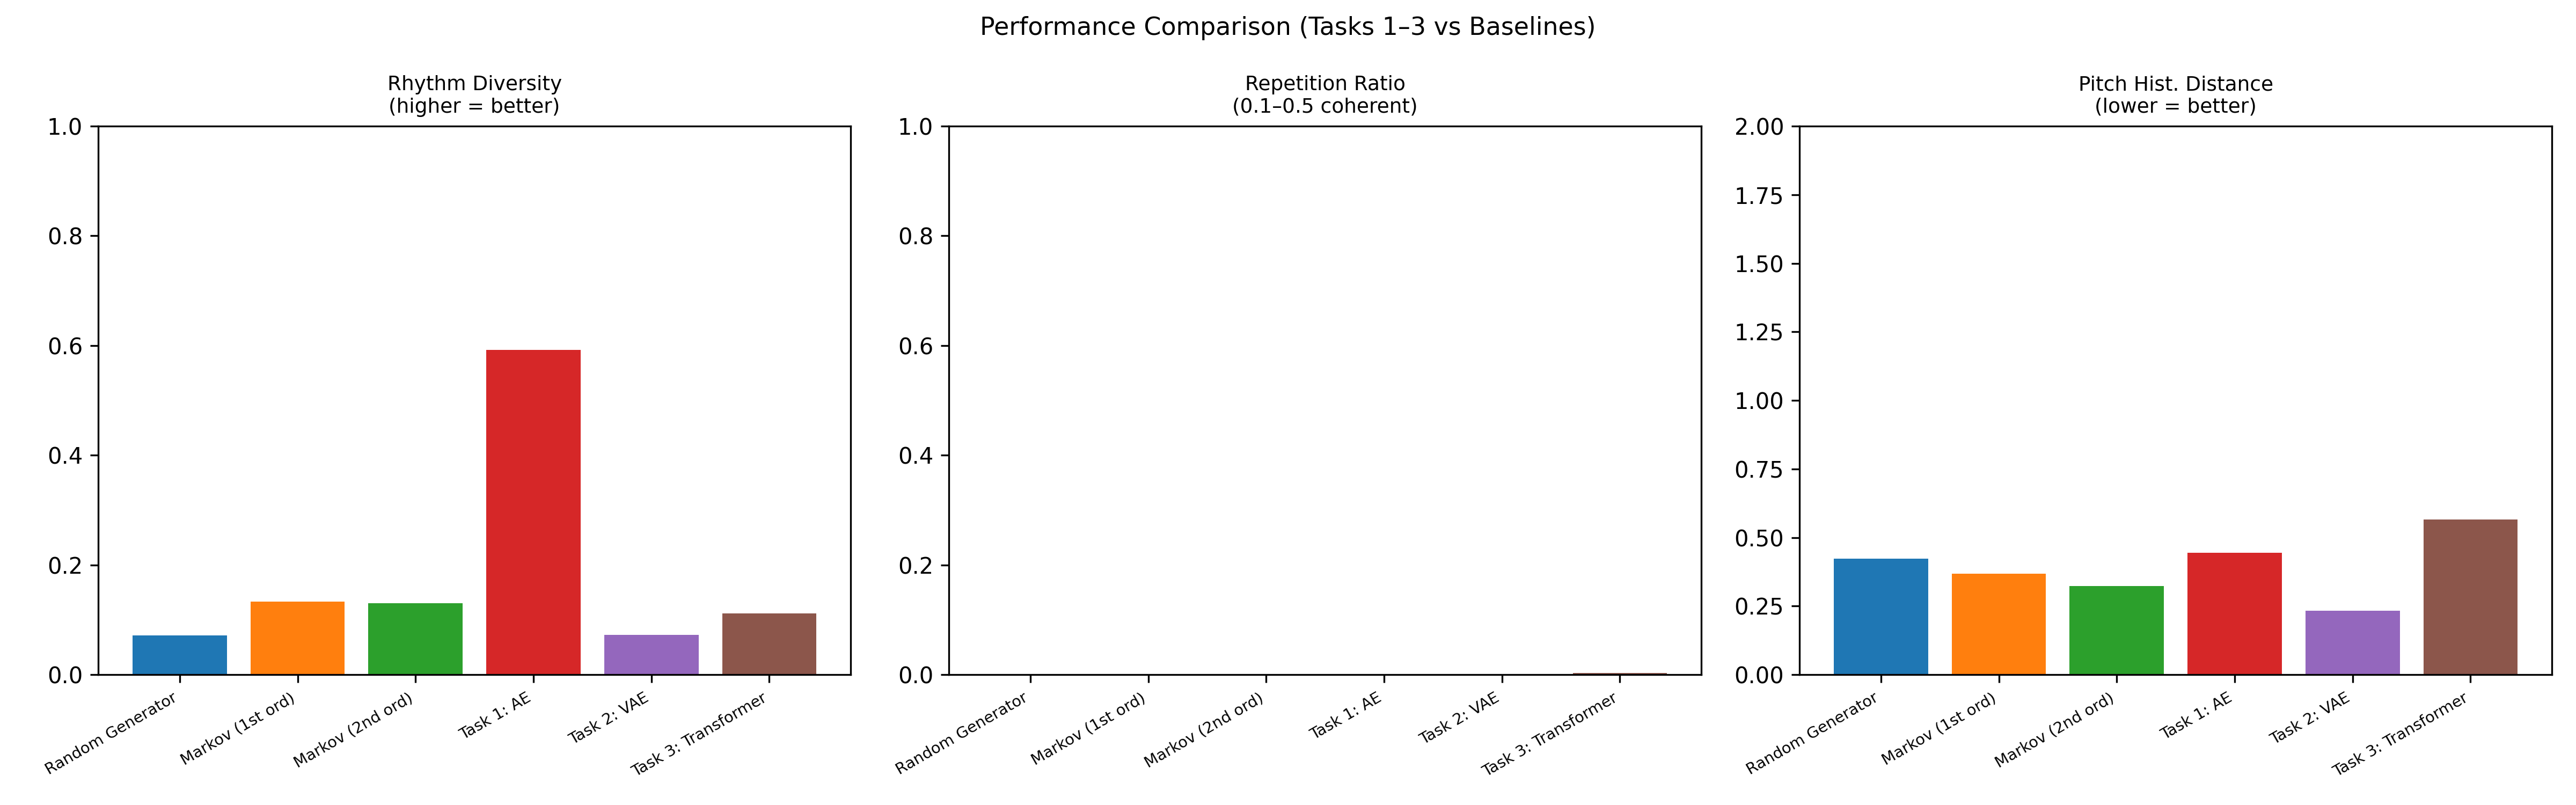
\includegraphics[width=\columnwidth]{comparison_table.png}
\caption{Bar chart comparison of rhythm diversity, repetition ratio, and pitch histogram distance across all models. Pitch histogram distance y-axis spans 0--2 (lower is better); others span 0--1.}
\label{fig:comparison}
\end{figure}

\subsection{Task 1 vs.\ Task 2: AE and VAE Comparison}

Table~\ref{tab:ae_vae} provides a direct comparison between the LSTM AE and VAE on shared metrics. Although both architectures use identical encoder–decoder backbones and the same Focal Loss for reconstruction, the VAE's probabilistic latent space introduces two key differences.

\begin{table}[t]
\caption{Direct Comparison: Task~1 (AE) vs.\ Task~2 (VAE)}
\label{tab:ae_vae}
\begin{center}
\begin{tabular}{l c c}
\toprule
\textbf{Metric} & \textbf{AE} & \textbf{VAE} \\
\midrule
Parameters            & 1.78M  & 1.79M  \\
Best val loss         & 0.0986 & 0.2251 \\
Best epoch            & 50/50  & 7/50   \\
Rhythm diversity $\uparrow$     & 0.5916 & 0.0730 \\
Repetition ratio      & 0.0000 & 0.0000 \\
Pitch hist.\ distance $\downarrow$ & 0.4441 & 0.2328 \\
Pitch entropy         & 0.9481 & 0.9981 \\
Generated samples     & 5      & 8 + 8 interp. \\
Output duration       & 8.0~s  & 8.0~s  \\
Note range            & 51--72 & 54--70 \\
Latent interpolation  & No     & Yes    \\
\bottomrule
\end{tabular}
\end{center}
\end{table}

\textbf{Reconstruction loss.} The AE has a lower validation Focal Loss (0.0986 vs.\ 0.2251) because it only optimizes the reconstruction. The VAE also incurs a total loss, which incorporates the $\beta$-weighted KL term; the reconstruction loss does not improve past epoch 7, while the growth of the KL loss increases the total loss.

\textbf{Pitch quality.} The generated pitch-class distribution from the VAE has a significantly lower pitch histogram distance (0.2328 vs.\ 0.4441), which results in a pitch-class distribution in closer alignment with real MAESTRO music. The KL regularisation term pushes the latent space towards $\mathcal{N}(0,\mathbf{I})$ so that the encoder does not fall into a degenerate posterior distribution; this way, at generation, the pitch distribution is more natural.

\textbf{Rhythm diversity.} The AE scores markedly higher (0.5916 vs.\ 0.0730). This is a consequence of the increased reconstruction uncertainty that arises with the AE decoder, as different latent samples lead to greater frame-by-frame activations without KL regularisation. The VAE is more restricted and thus generates more uniform and smoother rhythmic patterns from previous samples.

\textbf{Latent structure.} The VAE uniquely supports latent interpolation. Decoding $\mathbf{z}_\alpha = (1{-}\alpha)\boldsymbol{\mu}_1 + \alpha\boldsymbol{\mu}_2$ across 8 steps produces perceptually gradual transitions between two encoded real pieces, confirming that the KL annealing strategy successfully organises the latent space without posterior collapse.

\subsection{Generated Output Quality}

All of the MIDI files generated met the minimum requirements (50 notes, 5 seconds). The AE and VAE create 8-second (input window length) piano-roll windows, and the Transformer creates a sequence of windows 13--32 seconds long that generate 512 new tokens autoregressively.

Qualitative examination shows that the output of AE tends to be denser with chords (more notes at the same time in the output) when uncertainty is high, which happens when the decoder is tempted to fire multiple pitches at the same time. The outputs of VAE are perceptually smoother and the latent interpolation experiment (midway between two encoded real pieces using 8 intermediate MIDI files) demonstrates that stylistic transitions between the pieces are gradual instead of abrupt, which is evidence that the KL annealing successfully structured the latent space.

The note-level structure in transformer outputs is most natural, with clearly marked bar boundaries, as well as variations in velocity and occasional longer-range patterns. Greedy decoding would cause degenerate repetition loops which are avoided by top-$k$ sampling ($k{=}50$ and temperature 1.1).

All generated MIDI files (AE samples, VAE samples and latent interpolations, Transformer samples) are publicly available for listening at:
\begin{center}
\url{https://drive.google.com/drive/folders/1n7gyIyUzjG9LVD5ZzIh4z1M-wgBidOEe?usp=sharing}
\end{center}

\subsection{Baseline Comparison}

\begin{figure}[t]
\centering
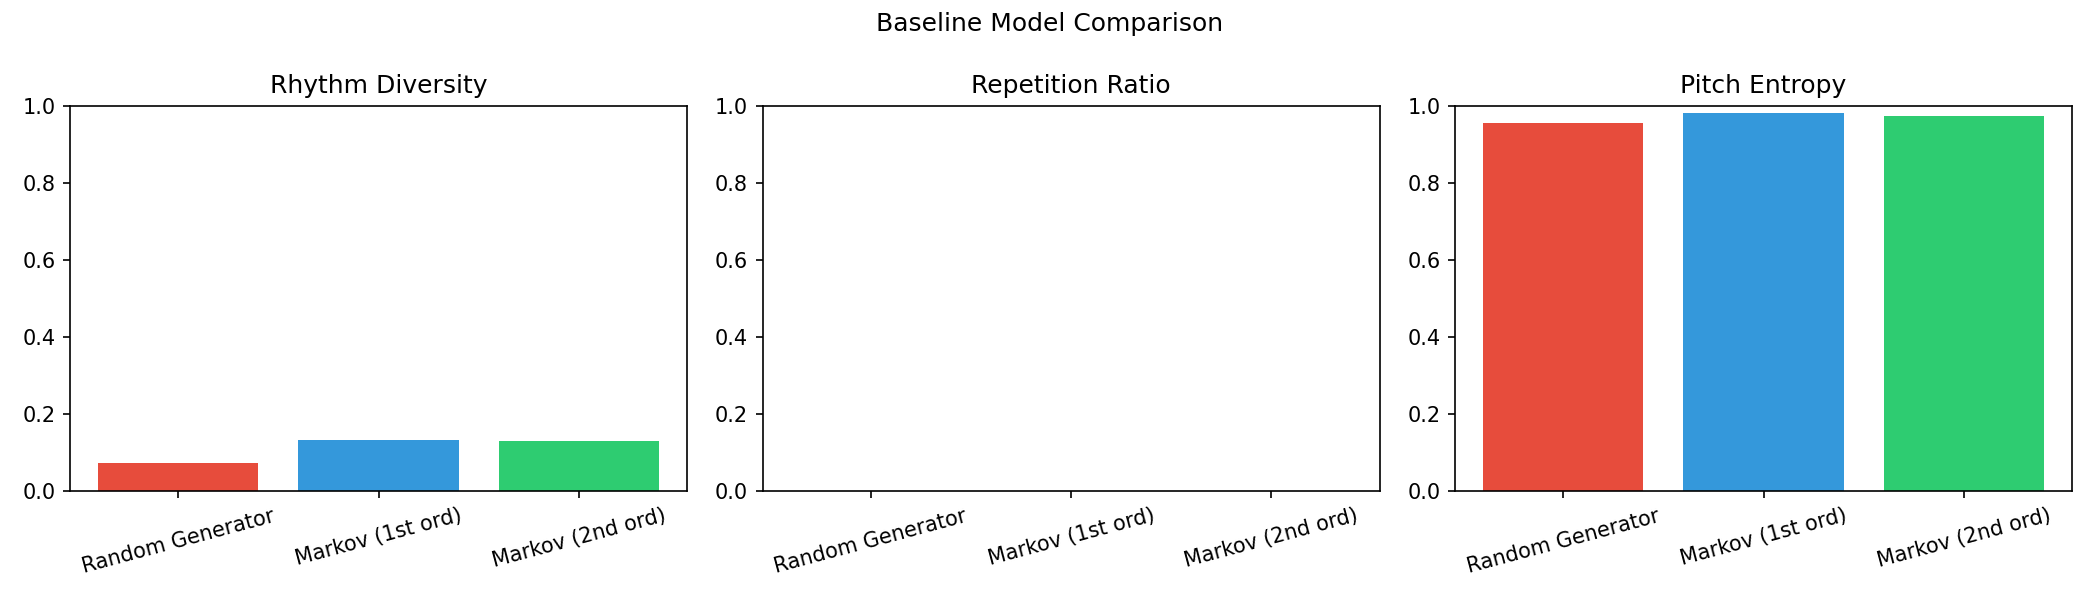
\includegraphics[width=\columnwidth]{baseline_comparison.png}
\caption{Quantitative evaluation of baseline models (Random Generator, Markov 1st and 2nd order) across rhythm diversity, repetition ratio, and pitch entropy metrics.}
\label{fig:baseline}
\end{figure}

The random generator, although high pitch entropy (0.954), has no melodic coherence as all notes are independent. The first-order Markov chain is able to reflect local pitch changes, but it results in monotonically decreasing rhythm variety compared to the random baseline because of its empirical duration model that focuses probability mass on common durations. The lower pitch histogram distance of the second-order chain (0.3230 vs. 0.3691) also shows that the bigram pitch context is closer to the actual pitch class distribution.

All the three learned models achieve higher pitch histogram similarity (Task~2 VAE) or higher rhythmic variety (Task~1 AE, Task~3 Transformer) than the baselines, which confirms the usefulness of unsupervised deep learning over statistical baselines for this task.

% ============================================================
\section{Conclusion}
\label{sec:conclusion}

We proposed and compared three unsupervised generative models in generating symbolic piano music: LSTM Autoencoder, Variational Autoencoder with KL annealing, and decoder-only Transformer trained on REMI token sequences. The AE has a deterministic reconstruction at a quick speed, the VAE brings in stochasticity and a structured latent space for interpolation and the Transformer has the most natural long-range sequential structure at a higher training complexity.

The VAE best approximates the real pitch-class distributions (pitch histogram distance 0.2328), the Transformer yields the most musically varied long-form outputs, and the only non-trivial repetition ratio among the learned models is the one achieved by the Transformer. They both outperform the random and Markov baselines on at least one metric.

Due to hardware time constraints, the Transformer was trained for 20 epochs (as opposed to 50 epochs) and the perplexity could be reduced further. The models are trained only on classical piano (MAESTRO), thus with restricted genre diversity. The high score of the AE's rhythm diversity is a result of the representation of the piano-roll at the frame level and not of real musical diversity.

There are several avenues for future work, such as training on multi-genre MIDI corpora (Lakh MIDI Dataset), applying the relative position encodings to the Transformer to further enhance long-range coherence, and using reinforcement learning from human feedback (RLHF) to fine-tune generation quality to better match preferences of human listeners.

% ============================================================

\begin{thebibliography}{00}

\bibitem{maestro}
C. Hawthorne, A. Stasyuk, A. Roberts, I. Simon, C.-Z. A. Huang, S. Dieleman, E. Elsen, J. Engel, and D. Eck,
``Enabling factorized piano music modeling and generation with the MAESTRO dataset,''
in \textit{Proc. ICLR}, 2019.

\bibitem{vae}
D. P. Kingma and M. Welling,
``Auto-encoding variational Bayes,''
in \textit{Proc. ICLR}, 2014.

\bibitem{transformer}
A. Vaswani, N. Shazeer, N. Parmar, J. Uszkoreit, L. Jones, A. N. Gomez, L. Kaiser, and I. Polosukhin,
``Attention is all you need,''
in \textit{Advances in Neural Information Processing Systems}, vol. 30, 2017.

\bibitem{musetransformer}
Y.-S. Huang and Y.-H. Yang,
``Pop music transformer: Beat-based modeling and generation of expressive pop piano compositions,''
in \textit{Proc. ACM MM}, 2020.

\bibitem{miditok}
N. Fradet, J.-P. Briot, F. Chhel, A. El Fallah Seghrouchni, and N. Gutowski,
``MidiTok: A Python package for MIDI file tokenization,''
in \textit{Proc. ISMIR Late-Breaking Demo}, 2021.

\bibitem{prettymidi}
C. Raffel and D. P. W. Ellis,
``Intuitive analysis, creation and manipulation of MIDI data with \texttt{pretty\_midi},''
in \textit{Proc. ISMIR Late-Breaking Demo}, 2014.

\bibitem{focal}
T.-Y. Lin, P. Goyal, R. Girshick, K. He, and P. Dollar,
``Focal loss for dense object detection,''
in \textit{Proc. ICCV}, 2017, pp. 2980--2988.

\bibitem{musicvae}
A. Roberts, J. Engel, C. Raffel, C. Hawthorne, and D. Eck,
``A hierarchical latent vector model for learning long-term structure in music,''
in \textit{Proc. ICML}, 2018.

\bibitem{lakh}
C. Raffel,
``Learning-based methods for comparing sequences, with applications to audio-to-MIDI alignment and matching,''
Ph.D. dissertation, Columbia University, 2016.

\end{thebibliography}

\end{document}
